\subsection{Discriminative learning and task-ID residual gates}
The selected CSA paper also evaluates discriminative processing after tensor representation~\cite{csa}. We therefore test whether regularized LDA can improve expert selection from the frozen CSA cores. CSA bases are unchanged and remain reconstruction-trained; LDA changes the downstream supervised objective. All seven CSA ranks, corresponding PCA controls, raw delta and base features use identical new method grids. This is an exploratory follow-up to inspected final results.

LDA uses empirical class priors and shared covariance
\[
 \Sigma_\alpha=(1-\alpha)S_w+\alpha\,\frac{\operatorname{tr}(S_w)}{D}I,
 \qquad \alpha\in\{0.1,0.5,0.9\}.
\]
Its linear discriminant is implemented with a dual solve for high-dimensional raw features and checked against the standard scikit-learn shrinkage-LDA implementation. A small diagonal floor handles zero within-class variance. Scaling uses fit data only; known-task one-hot features are then appended.

We compare three rules. \emph{Direct LDA} predicts the minimum-ground-truth-NLL expert. \emph{Task prior} keeps the own expert unless an alternative's predicted probability exceeds the own expert's probability by a selection-chosen margin. \emph{Benefit LDA} predicts help, tie or harm relative to the own expert for each alternative, and switches only if $P(\text{help})-P(\text{harm})$ exceeds a chosen threshold. An expert's own-task examples have identically zero benefit, so they are excluded from its benefit-classifier fit; each such classifier uses 384 examples. These posteriors are model estimates, not established calibrated guarantees.

Direct LDA chooses shrinkage by selection native score. Both gated families include always-own and require selection native and macro accuracy at least task ID, with worst accuracy no more than 0.01 lower. Among eligible candidates we maximize native, then macro accuracy, then minimize switching; ties prefer always-own and stronger regularization. These are selection constraints rather than guarantees on final data. All choices lock before reading the internal final. Every candidate's selection routes and the selected final routes are independently reloaded and recomputed.

\begin{table}[htbp]\centering\scriptsize
\caption{Discriminative follow-up on the same internal final, three fixed teacher seeds. All candidates use matched grids across representations. Switch/help/harm are mean percentages; native score is mean $\pm$ sample SD. Own is the number of seeds selecting always-own.}
\begin{tabular}{llrrrrr}\toprule
Features & Method & Native & Switch & Help & Harm & Own \\ \midrule
task\_id & reference & 0.7695 $\pm$ 0.0114 & 0.00 & 0.00 & 0.00 & 3/3 \\
csa2x8 & previous\_logistic & 0.7080 $\pm$ 0.0250 & 19.43 & 1.30 & 3.71 & 0/3 \\
csa2x8 & direct\_lda & 0.7485 $\pm$ 0.0290 & 11.49 & 0.65 & 1.20 & 0/3 \\
csa2x8 & task\_prior & 0.7695 $\pm$ 0.0114 & 0.00 & 0.00 & 0.00 & 3/3 \\
csa2x8 & benefit\_lda & 0.7695 $\pm$ 0.0114 & 0.00 & 0.00 & 0.00 & 3/3 \\
pca16 & benefit\_lda & 0.7652 $\pm$ 0.0177 & 0.39 & 0.07 & 0.20 & 2/3 \\
pca3 & benefit\_lda & 0.7662 $\pm$ 0.0161 & 0.42 & 0.03 & 0.13 & 2/3 \\
raw\_delta & benefit\_lda & 0.7695 $\pm$ 0.0114 & 0.00 & 0.00 & 0.00 & 3/3 \\
\bottomrule\end{tabular}\end{table}

At the fixed CSA $2\times8$ setting, direct LDA has native score 0.7485, versus 0.7080 for the earlier logistic router and 0.7695 for task-ID selection.

The task-prior gate has native score 0.7695; it chooses always-own in 3/3 seeds and makes nonzero final switches in 0/3. Mean switched, helped and harmed fractions are 0.000\%, 0.000\%, and 0.000\%, respectively. Its macro-accuracy change versus task ID is +0.000 percentage points.

The benefit-LDA gate has native score 0.7695; it chooses always-own in 3/3 seeds and makes nonzero final switches in 0/3. Mean switched, helped and harmed fractions are 0.000\%, 0.000\%, and 0.000\%, respectively. Its macro-accuracy change versus task ID is +0.000 percentage points.

These outcomes distinguish discriminative fitting, conservative fallback and actual useful switching. Matching the reference with zero switches is baseline preservation rather than evidence of learned routing benefit. Selection constraints alone do not establish final safety or a statistically significant improvement.


\begin{figure}[htbp]\centering
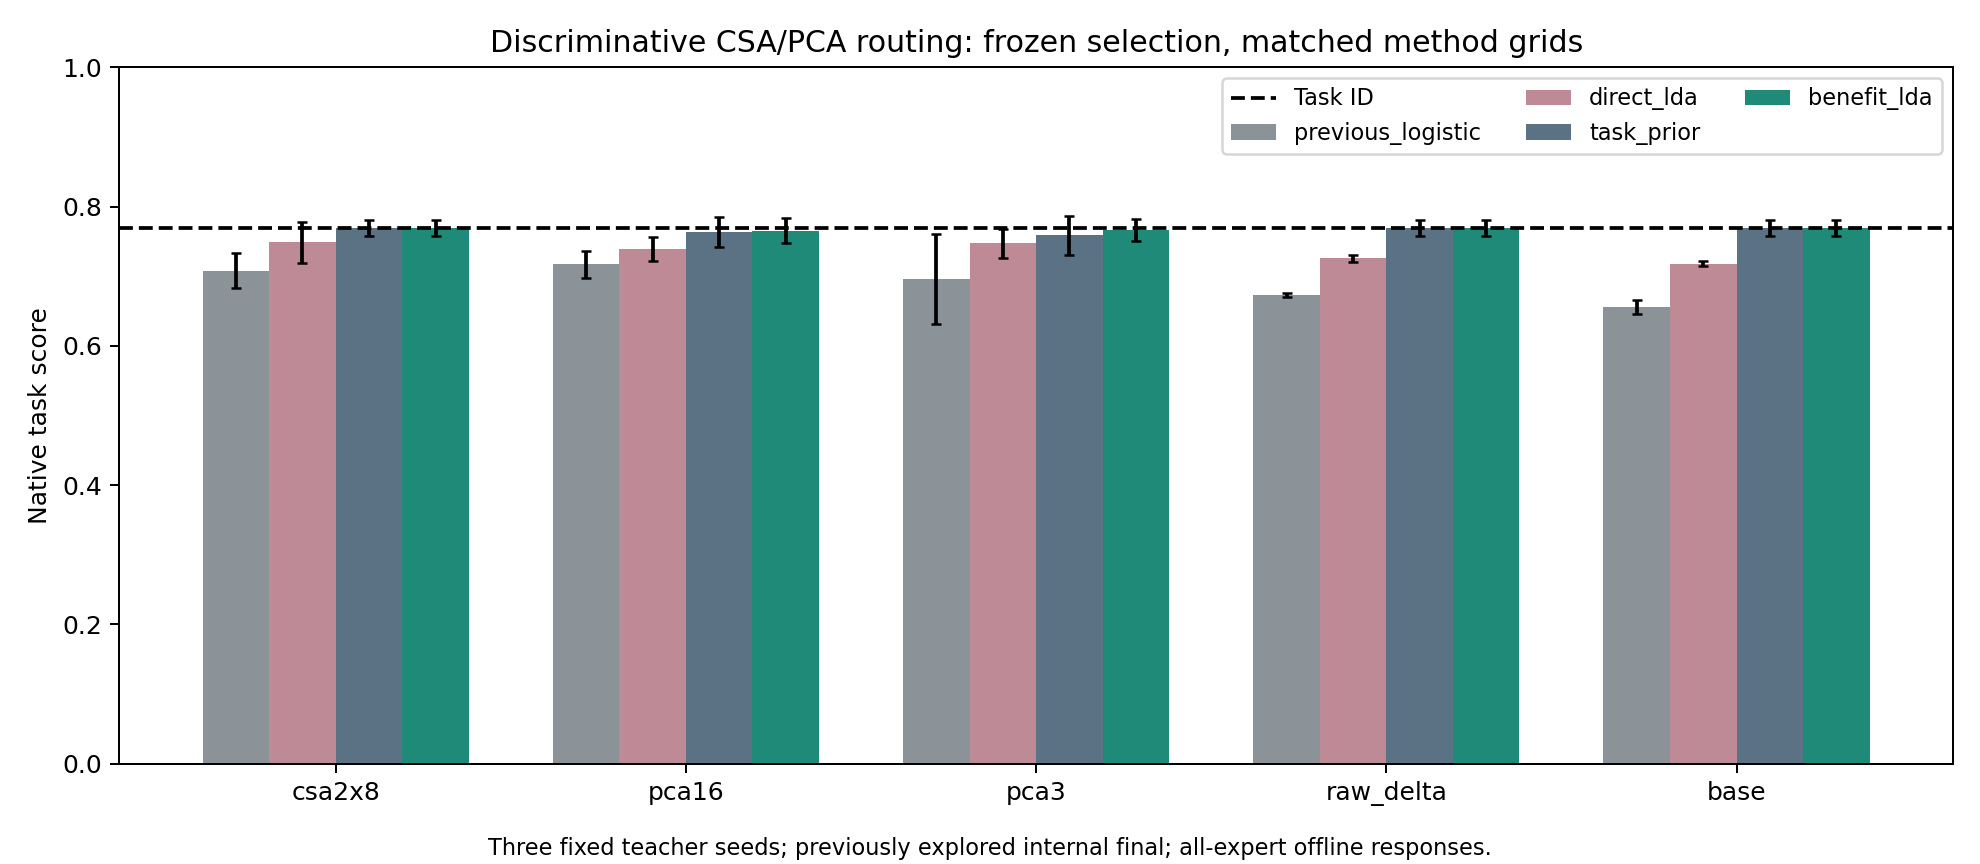
\includegraphics[width=\linewidth]{../artifacts/csa-discriminant-2026-11-11/discriminant-quality.png}
\caption{Discriminative and residual-gating controls on fixed representations. Error bars show sample SD across the same three teacher seeds. Matching task ID by selecting always-own is distinguished from learning useful switches; actual help/harm records accompany the results.}
\end{figure}

All-expert responses are still required. Thus any improvement here concerns offline information use, not reduced serving cost. The native score combines task-specific metrics; helped minus harmed equals the macro-accuracy change, rather than the native-score change. We report the full frozen rank grid and do not replace the illustrative rank by a final-selected winner.
